\documentclass[12pt]{article}
\usepackage{amssymb}
\usepackage[utf8]{inputenc}
\usepackage{amsmath}
\usepackage{parskip}
\usepackage[a4paper,margin=2cm]{geometry}
\usepackage{graphicx}
\usepackage{float}
       
\title{\textbf{Laboratorio 1 de Analisis de Señales y Sistemas}}
\author{lunayabarrena }
\date{4 de Julio del 2021}

\begin{document}
\maketitle

Sea $f(t)=u(t)-u(t-3)$ la señal pulso rectangular , $g(t)= e^{-2t}u(t) , 0\leq t\leq 5$ la  amortiguacion exponencial y sea $h(t)$ la señal  pulso triangular definida asi :

\[h(t)=\left\{ \begin{array}{lccc}
             0 &   si  & t \leq 0 \\
             \\ t &  si & 0 < t < 1 \\
             \\ 2-t &  si  & 1 < t < 2\\
             \\  0 & si &  t < 2
             \end{array}
   \right.
\]
Usando el MATLAB grafique las señales  en tiempo continuo $f(t) , g(t) , h(t)$\newline
Encuentre en terminos de  de t y de la señal escalon  unitario  las siguientes convoluciones: $f(t)*g(t) ,f(t)*h(t) ,g(t)*h(t)\newline  $
Usando el matlab y el comando \textit{conv} grafique las convoluciones $f(t)*f(t),\ f(t)*g(t), \ g(t)*g(t),\ g(t)*h(t),\ h(t)*h(t)$.\newline


\textbf{funcion f(t)=u(t)-u(t-3)=rectpuls(t-1.5)}
\begin{figure}[H]
    \centering
    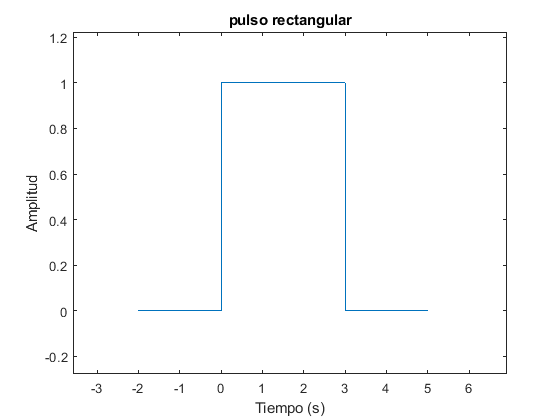
\includegraphics[scale=0.80]{fig1.png}
    \caption{grafica de la funcion f(t)}
    \label{fig:my_label}
\end{figure}



\textbf{funcion $g(t)=e^{-2t}u(t)$}
\begin{figure}[H]
    \centering
    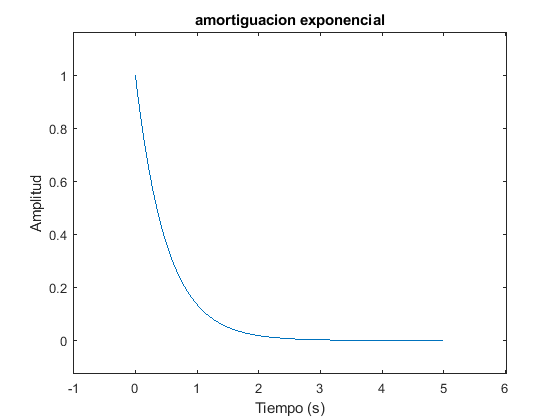
\includegraphics[scale=0.80]{fig2.png}
    \caption{grafica de la funcion g(t)}
    \
\end{figure}



\textbf{funcion $h(t)= \ tripuls(t-1) \ = u_1(t)-2u_1(t-1)+u_1(t-2) $}
\begin{figure}[H]
    \centering
    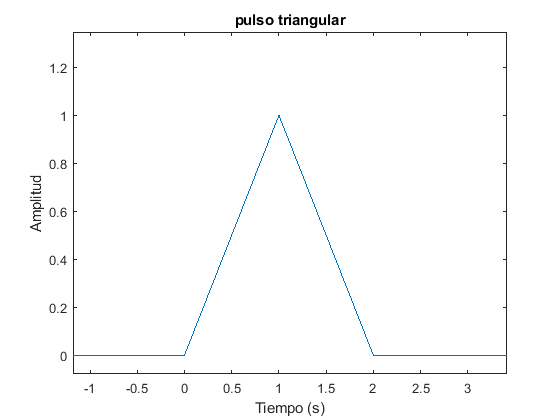
\includegraphics[scale=0.80]{fig3.png}
    \caption{grafica de la funcion g(t)}
\end{figure}
\newpage



Ahora hallaremos las convoluciones de \ $f(t)*g(t) ,f(t)*h(t) ,g(t)*h(t)$\newline \newline
\empty{\underline{\textbf{$f(t)*g(t)$= $\int_{-\infty}^{\infty} g(\tau)f(t-\tau) d\tau  $}}}
\newline$\\
Para  \ t<0$
\begin{figure}[H]
    \centering
    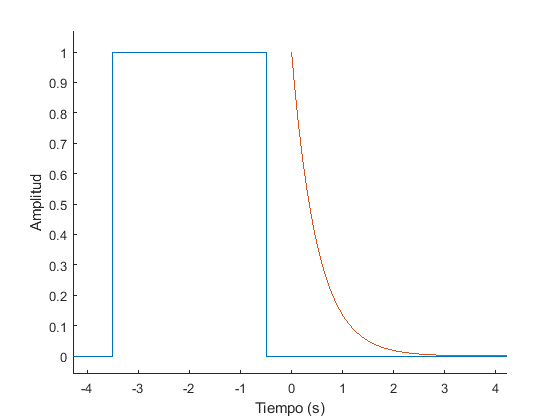
\includegraphics[scale=0.7]{fig4.png}
    \caption{para valores de $ t\ < 0$}
    \label{fig:my_label}
\end{figure}

Vemos que las graficas no se interceptan , por lo tanto $\int_{-\infty}^{\infty} g(\tau)f(t-\tau) d\tau = 0 $\newline


Para   $0 < t < 3$ \\
\begin{figure}[H]
    \centering
    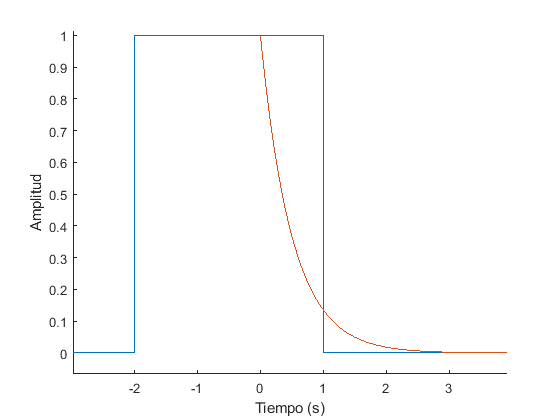
\includegraphics[scale=0.6]{fig5.png}
    \caption{grafica en $0 < t < 3$ }
\end{figure}
$\int_{-\infty}^{\infty} g(\tau)f(t-\tau) d\tau = \int_{0}^{t} e^{-2t}.1 d\tau = \dfrac{1}{2}-\dfrac{e^{-2t}}{2}  $\\
\newpage


Para   $3 < t < 5$ \\
\begin{figure}[H]
    \centering
    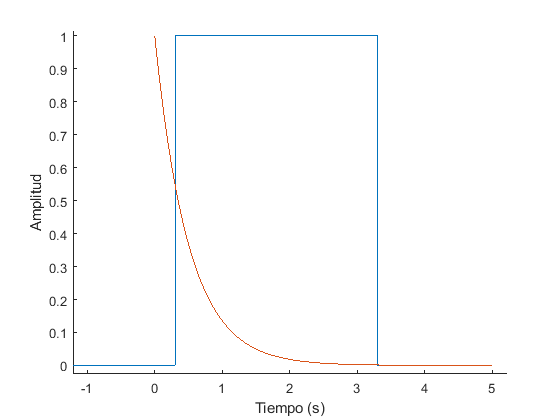
\includegraphics[scale=0.6]{fig6.png}
    \caption{grafica en $3 < t < 5$ }
\end{figure}
$\int_{-\infty}^{\infty} g(\tau)f(t-\tau) d\tau = \int_{-3+t}^{t} \ e^{-2t}.1 d\tau = \ \dfrac{e^{-2t+6}}{2}-\dfrac{e^{-2t}}{2}  $\\
\newline
\newline


Para   $5 < t < 8$ \\
\begin{figure}[H]
    \centering
    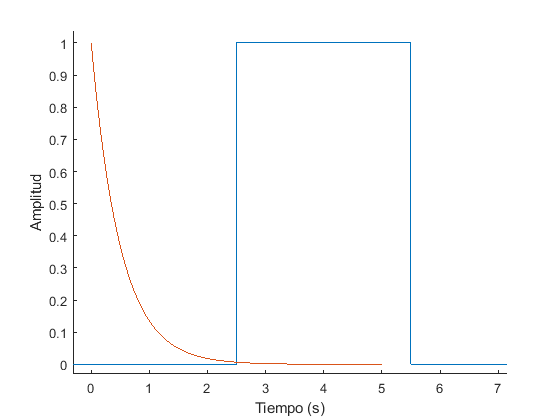
\includegraphics[scale=0.6]{fig7.png}
    \caption{grafica en $5 < t < 8$ }
\end{figure}
$\int_{-\infty}^{\infty} g(\tau)f(t-\tau) d\tau = \int_{-3+t}^{5} \ e^{-2t}.1 d\tau = \ \dfrac{e^{-2t+6}}{2}-\dfrac{e^{-10}}{2}  $\\
\newpage



Para   $8 < t$ \\
\begin{figure}[H]
    \centering
    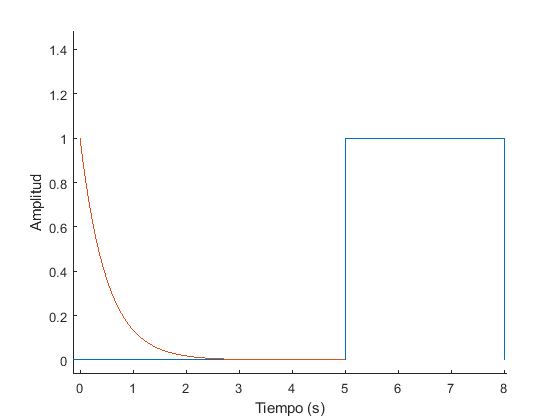
\includegraphics[scale=0.6]{fig8.png}
    \caption{grafica en $5 < t < 8$ }
\end{figure}

$\int_{-\infty}^{\infty} g(\tau)f(t-\tau) d\tau = \int_{8}^{\infty} \ e^{-2t}.1 d\tau = 0  $\\ \newline
la grafica de $f(t)*g(t)$ es

\begin{figure}[H]
    \centering
    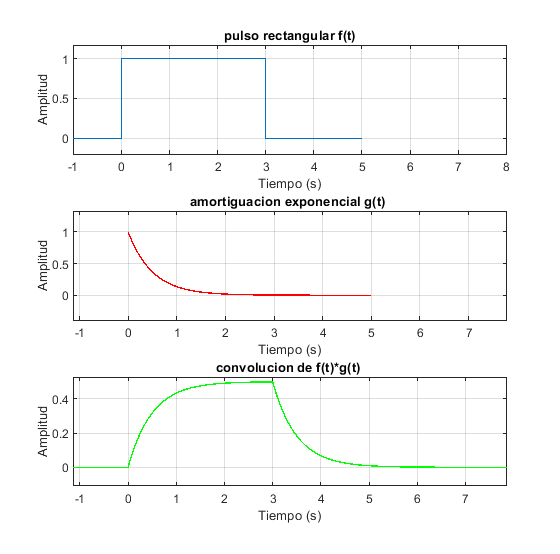
\includegraphics[scale=0.8]{fig9.png}
    \caption{convolucion de $f(t)*g(t)$ }
\end{figure}
\newpage










\empty{\underline{\textbf{$f(t)*h(t)$= $\int_{-\infty}^{\infty} h(\tau)f(t-\tau) d\tau  $}}}\newline


sabemos que :\newline \newline
$u_{n}(t)*u_{m}(t)=u_{n+m+1}(t)$\newline
$u_{n}(t-a)*u_{m}(t-b)=u_{n+m+1}(t-a-b)$\newline\newline
$f(t)=rectpuls(t-1.5)\ = u_0(t)-u_0(t-3)$\newline 
$h(t)=tripuls(t-1) \ = u_1(t)-2u_1(t-1)+u_1(t-2)$\newline 

$f(t)*h(t)=(u_0(t)-u_0(t-3))*(u_1(t)-2u_1(t-1)+u_1(t-2))$\newline
$f(t)*h(t) \ =u_2(t)-2u_2(t-1)+u_2(t-2)-u_2(t-3)+2u_2(t-4)-u_2(t-5)$\newline \newline
la grafica de $f(t)*h(t) es $

\begin{figure}[H]
    \centering
    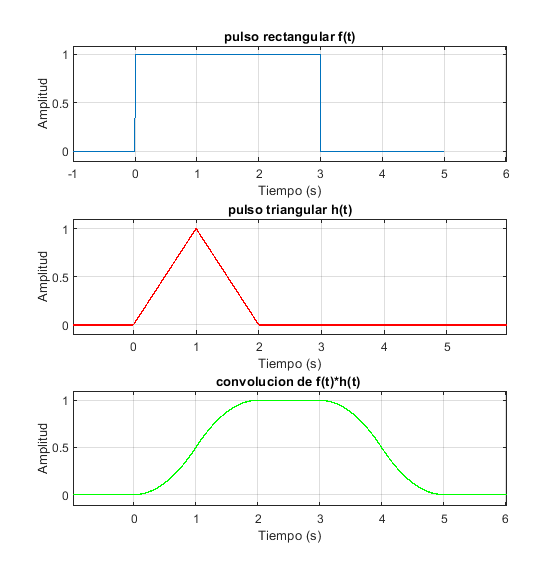
\includegraphics[scale=0.9]{fig10.png}
    \caption{convolucion de $f(t)*h(t)$ }
\end{figure}  \newpage
la grafica de $g(t)*h(t)$\newline \newline
\begin{figure}[H]
    \centering
    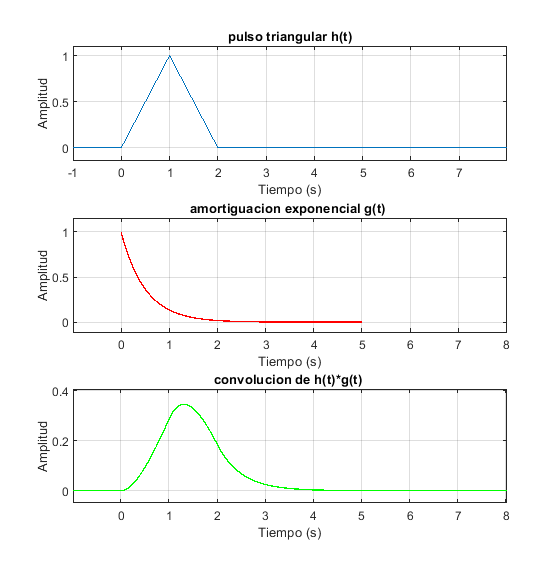
\includegraphics[scale=1.1]{fig11.png}
    \caption{convolucion de $f(t)*h(t)$ }
\end{figure}
\newpage










Ahora usando \textbf{matlab} y el comando \textit{conv}  hallaremos las convoluciones de $f(t)*f(t),\ f(t)*g(t), \ g(t)*g(t),\ g(t)*h(t),\ h(t)*h(t)$
\newline \newline
\textbf{$f(t)*f(t)$}
\begin{figure}[H]
    \centering
    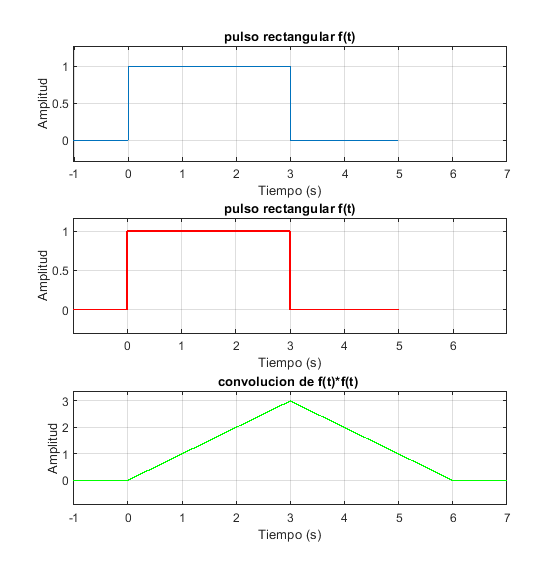
\includegraphics[scale=1.2]{fig12.png}
    \caption{convolucion de $h(t)*h(t)$ }
\end{figure}
\newpage
\textbf{$f(t)*g(t)$}
\begin{figure}[H]
    \centering
    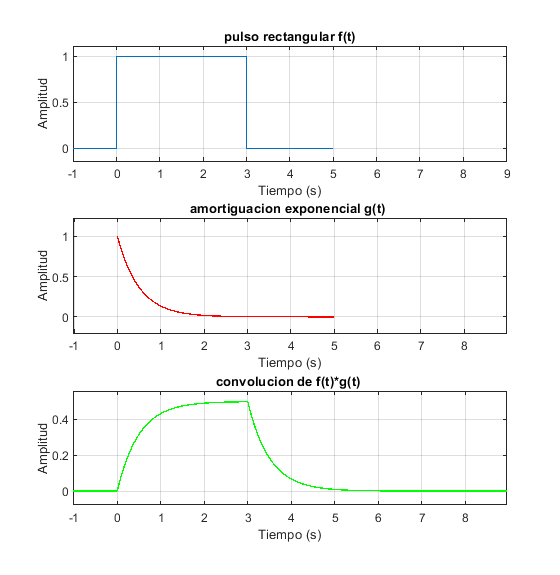
\includegraphics[scale=1.2]{fig13.png}
    \caption{convolucion de $f(t)*h(t)$ }
\end{figure}
\newpage
\textbf{$g(t)*g(t)$}
\begin{figure}[H]
    \centering
    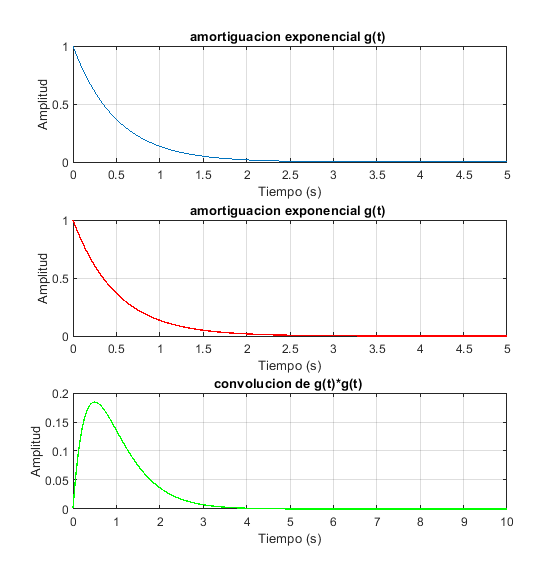
\includegraphics[scale=1.2]{fig14.png}
    \caption{convolucion de $g(t)*g(t)$ }
\end{figure} 
\newpage
\textbf{$g(t)*h(t)=h(t)*g(t)$}
\begin{figure}[H]
    \centering
    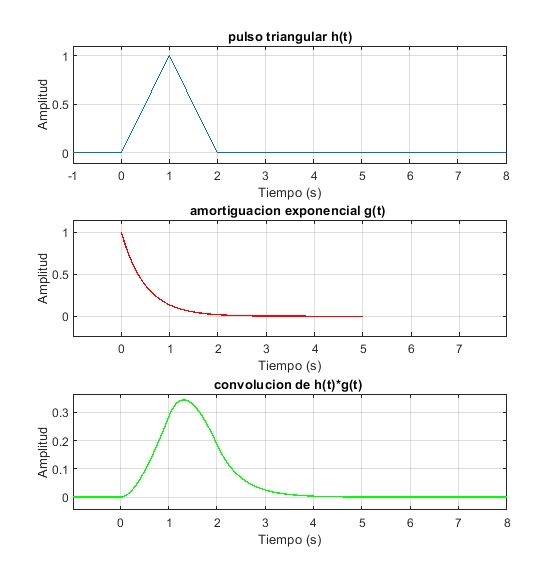
\includegraphics[scale=1.2]{fig15.png}
    \caption{convolucion de $g(t)*g(t)$ }
\end{figure} 
\newpage
\textbf{$h(t)*h(t)=h(t)*h(t)$}

\begin{figure}[H]
    \centering
    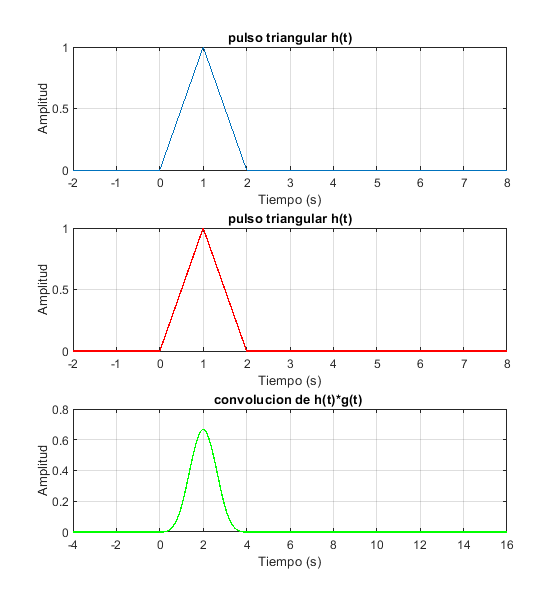
\includegraphics[scale=1.2]{fig16.png}
    \caption{convolucion de $h(t)*g(t)$ }
\end{figure}









\end{document} 